\documentclass[10pt]{book}
\usepackage{gvv-book}                                
\usepackage{gvv} 
\usepackage[sectionbib,authoryear]{natbib}% for name-date citation comment the below line
\usepackage{setspace} 
\setstretch{1.0}
\setcounter{secnumdepth}{3} 
\setcounter{tocdepth}{2}
\makeindex
\let\cleardoublepage\clearpage
\begin{document}
\frontmatter
%%%%%%%%%%%%%%%%%%%%%%%%%%%%%%%%%%%%%%%%%%%%%%%%%%%%%%%%%%%%%%%%
\booktitle{Geometry}
\subtitle{Through Algebra}
\AuAff{Errala Paulsonashish}
%\halftitlepage
\titlepage
\tableofcontents
%\listoffigures %optional
%\listoftables  %optional
%% before \tableofcontents
%%%%%%%%%%%%%%%%%%%%%%%%%%%%%%%%%%%%%%%%%%%%%%%%%%%%%%%%%%%%%%%%
\setcounter{page}{0}
\begin{introduction}
This book shows how to solve problems in geometry using trigonometry and coordinate geometry.
\end{introduction}
\mainmatter
\chapter{Triangle}
Consider a triangle with vertices
                \begin{align}
                        \label{eq:tri-pts}
                        \vec{A} = \myvec{-5 \\ -4},\,
                        \vec{B} = \myvec{3 \\ -3},\,
                        \vec{C} = \myvec{4 \\ 0}
                \end{align}
\section{Vectors}
\begin{enumerate}[label=\thesection.\arabic*.,ref=\thesection.\theenumi]
\numberwithin{equation}{enumi}
\item The direction vector of $\vec{AB}$ is defined as
\begin{align}
    \vec{B}-
    \vec{A}
\end{align} 
 Find the direction vectors of $\vec{AB}, \vec{BC}$ and $\vec{CA}$.\\
\solution\\
\begin{enumerate}
\item The direction vector of $\vec{AB}$ is
\begin{align}
    &= \vec{B}- \vec{A}\\ &= \myvec{ 3 - (-5)\\ -3 -(-4)}\\ &= \myvec{ 8 \\ 1}
    \label{eq:geo-dir-vec-ab}
\end{align}
\item The direction vector of $\vec{BC}$ is
\begin{align}
    &= \vec{C}- \vec{B}\\ &= \myvec{ 4 - (3)\\ 0 -(-3)}\\ &=\myvec{ 1 \\ 3}
    \label{eq:geo-dir-vec-bc}
\end{align}
\item The direction vector of $\vec{CA}$ is
\begin{align}
    &= \vec{A}- \vec{C}\\ &= \myvec{ -5 - (4)\\ -4 -(0)}\\ &=\myvec{ -9 \\ -4}
    \label{eq:geo-dir-vec-ca}
\end{align}
\end{enumerate}
\item The length of side $\vec{BC}$ is
\begin{align}
\norm{\vec{B}-\vec{A}} \triangleq \sqrt{\brak{\vec{B}-\vec{A}}^{\top}{\vec{B}-\vec{A}}}
\end{align}\\
where,
\begin{align}
\begin{split}
\vec{A}^{\top}\triangleq\myvec{-5 & -4}
\end{split}
\end{align}
\solution \\
Given,\\
                \begin{align}
                \vec{A} = \myvec{-5 \\ -4},
                \vec{B} = \myvec{3 \\ -3},
                \vec{C} = \myvec{4 \\ 0}
                \end{align}
                \begin{align}
                \norm{\vec{B}-\vec{C}} \ &= \sqrt{\brak{\vec{B}-\vec{C}}^{\top}\brak{\vec{B}-\vec{C}}} \\
                \vec{B}-\vec{C} &= \myvec{3 \\ -3} - \myvec{4 \\ 0} \\
                \vec{B}-\vec{C} &= \myvec{-1 \\ -3} \\
                \brak{\vec{B}-\vec{C}}^{\top} &= {\myvec{-1 \\ -3}}^{\top} = \myvec{-1 \ -3} \\
                \brak{\vec{B}-\vec{C}}^{\top}\brak{\vec{B}-\vec{C}} &= \myvec{-1 \ -3} \myvec{-1 \\ -3} \\
                 & = 1 + 9 \\
                 & = 10 \\
                \sqrt{\brak{\vec{B}-\vec{C}}^{\top}\brak{\vec{B}-\vec{C}}} &= \sqrt{10} \\
                \label{eq:geo-norm-bc}
                 \implies \norm{\vec{B}-\vec{C}} &= \sqrt{10}
                \end{align}
Now solving for $\vec{AB}$,
\begin{align}
\vec{A}-\vec{B} &= \myvec{-8\\-1}\\
\norm{\vec{A}-\vec{B}} &= \sqrt{\myvec{-8 & -1}\myvec{-8\\-1}}\\
&= \sqrt{\brak{8}^2 +\brak{1}^2}\\
&=\sqrt{65}
\label{eq:geo-norm-ab}
\end{align}
Now solving for $\vec{CA}$,
    \begin{align}  
    	\vec{C}-\vec{A} &= \myvec{9\\4}\\
    	\norm{\vec{C}-\vec{A}} &= \sqrt{\myvec{9 & 4}\myvec{9\\4}}\\
        &= \sqrt{\brak{9}^2+\brak{4}^2}\\ &=\sqrt{97}
        \label{eq:geo-norm-ca}
    \end{align}
\item   Points $\vec{A}, \vec{B}, \vec{C}$ are defined to be collinear if
\begin{align}
\rank{\myvec{1 & 1 & 1 \\ \vec{A}& \vec{B}&\vec{C}}} = 2
\end{align}
Are the given points in
\eqref{eq:tri-pts}
collinear?
\\          
Question : Check the collinearity of $\vec{A},\vec{B},\vec{C}$
\\
\solution
Given that,
\begin{align}
    \vec{A} = \myvec{-5\\-4}
    \quad
    \vec{B} &= \myvec{3\\-3}
    \quad
    \vec{C} = \myvec{4\\0}
\end{align}
Given that $\vec{A},\vec{B},\vec{C}$ are collinear if
\begin{align}
    \text{rank}\myvec{
    1 & 1 & 1\\
    \vec{A} & \vec{B} & \vec{C} \\
    } &< 3
    \label{eq:1.1.3,2}
\end{align}
Let
\begin{align}
    \vec{R}&=\myvec{
    1 & 1 & 1
    \\
    -5 & 3 & 4
    \\
    -4 & -3 & 0
    }
\end{align}
The matrix $\vec{R}$ can be row reduced as follows,
\begin{align}
    \label{eq:matthrowoperations}
    \myvec{
    1 & 1 & 1
    \\
    -5 & 3 & 4
    \\
    -4 & -3 & 0
    }
     \xleftrightarrow[]{R_2 \leftarrow R_2+5R_1}
    \myvec{ 1 & 1 & 1
    \\
    0 & 8 & 9
    \\
    -4 & -3 & 0
    }
    \\
     \xleftrightarrow[]{R_3\leftarrow R_3+4R_1}
    \myvec{
    1 & 1 & 1
    \\
    0 & 8 & 9
    \\ 0 & 1 & 4
    }
    \\
     \xleftrightarrow[]{R_3\leftarrow R_3-R_2}
    \myvec{
    1 & 1 & 1
    \\
    0 & 8 & 9
    \\    
    0 & 0 & -5
    }
\end{align}
There are no zero rows. So,
\begin{align}
    \text{rank}\myvec{
    1 & 1 & 1\\
    \vec{A} & \vec{B} & \vec{C}\\
    } &= 3
\end{align}
Hence, from \eqref{eq:1.1.3,2} the points $\vec{A},\vec{B},\vec{C}$ are not collinear.
From Fig. \ref{fig1:Triangle}, We can see that $\vec{A},\vec{B},\vec{C}$ are not collinear .
\begin{figure}[H]
\centering
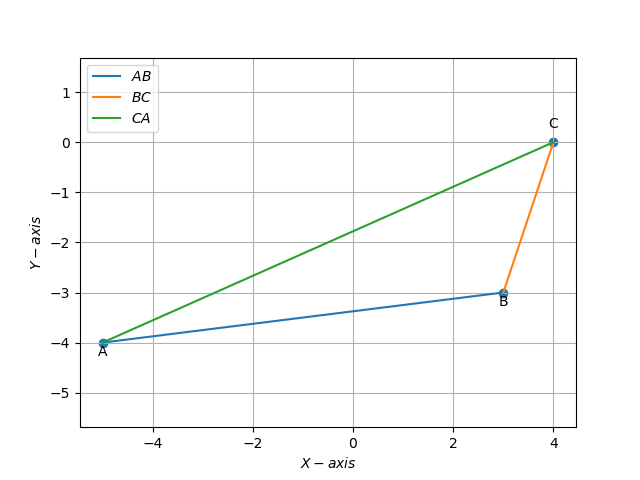
\includegraphics[width=\columnwidth]{figs/ABC_plot.png}
\caption{$\vec{A},\vec{B},\vec{C}$ plot}
\label{fig1:Triangle}
\end{figure}
\item The parameteric form of the equation  of $\vec{AB}$ is
                \begin{align}
                \label{eq:geo-param}
                \vec{x}=\vec{A}+k\vec{m}
                \end{align}
                where
                \begin{align}
		\vec{m}=\vec{B}-\vec{A}
                \end{align}
is the direction vector of $\vec{AB}$. Now Find the parameteric equations of $\vec{AB}, \vec{BC}$ and $\vec{CA}$.
\\  
\solution 
\begin{enumerate}
\item Parametric form of $\vec{AB}$ :
\begin{align}
\vec{x} = \vec{A} + k\vec{m}
\end{align}
where,
\begin{align}
\vec{m} = \vec{B} - \vec{A}
\end{align}
\begin{align}
\vec{B} - \vec{A} &= \myvec{3\\-3} - \myvec{ -5\\-4}\\
&= \myvec{3-(-5) \\ (-3)-(-4)}\\
\implies \vec {m} &= \myvec{8\\1}
\end{align}
therefore,
\begin{align}
\vec{AB} : \vec{x} &= \myvec{-5\\-4} + k\myvec{8\\1}
\end{align}
\item Parametric form of line $\vec{BC}$ :
\begin{align}
\vec{x} = \vec{B} + k\vec{m}
\end{align}
\begin{align}
\text{BC : } \vec{x} =& \myvec{3\\-3} + k\myvec{1\\3}
\end{align}
\item Parametric form of line $\vec{CA}$ :
\begin{align}
\vec{x} = \vec{C}+ k\vec{m}
\end{align}
\begin{align}
\text{CA : } \vec{x} =& \myvec{4\\0} + k\myvec{-9\\-4}
\end{align}
\end{enumerate}
 \item The normal form of the equation of $\vec{AB}$ is
\begin{align}
\vec{n}^{\top}\myvec{\vec{x}-\vec{A}}=0
\end{align}
where
\begin{align}
\vec{n}^{\top}\vec{m}&=\vec{n}^{\top}\myvec{\vec{B}-\vec{A}}=0
\end{align} 
or,\begin{align}
\vec{n}&=\myvec{0 &1 \\-1 & 0}\vec{m}
\end{align}
Find the normal form of the equations of $\vec{AB}$, $\vec{BC}$ and $\vec{CA}$\\
\solution:\\
       The normal equation for the side $\vec{AB}$ is
\begin{align}
\vec{n}^{\top}\myvec{\vec{x}-\vec{A}}&=0\\
\implies
\vec{n}^{\top}\vec{x}&=\vec{n}^{\top}\vec{A}
\end{align}
Now our task is to find the $\vec{n}$ so that we can find $\vec{n}^{\top}$.
As given. 
\begin{align}
  \vec{n} &= \myvec{0 & 1\\
  -1 & 0}\vec{m}
\end{align}
Here, $\vec{m} = \vec{B}- \vec{A}$ for side $\vec{AB}$
\begin{align}
\implies
\vec{m}&=\myvec{3\\-3} - \myvec{-5\\-4}\\
&=\myvec{8\\1}
\end{align}
Now as we have obtained vector $\vec{m}$.we can use this to obtain vector $\vec{n}$
\begin{align}
\vec{n} &= \myvec{0 & 1\\
  -1 & 0}\myvec{8\\1}
 = \myvec{1\\-8}
\end{align}
The transpose of $\vec{n}$ is
\begin{align}
  \vec{n}^{\top}&=\myvec{1 & -8}
\end{align}
Hence the normal equation of side $\vec{AB}$ is 
\begin{align}
    \myvec{1 & -8}\vec{x}&=\myvec{1 & -8}\myvec{-5\\-4}\\
    \implies \myvec{1 & -8}\vec{x} &= 27
\end{align}
\begin{figure}[H]
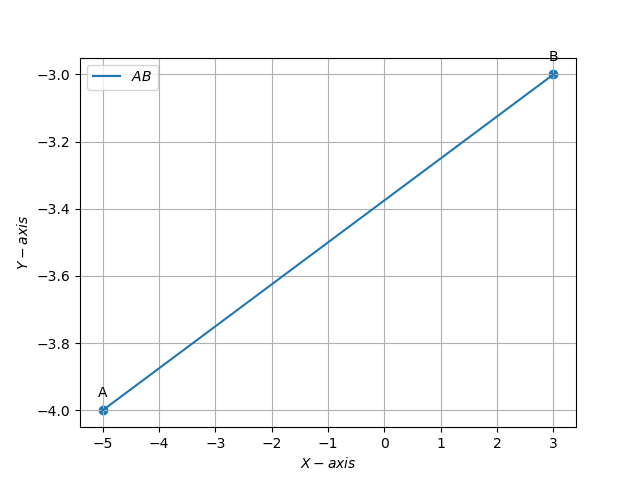
\includegraphics [width=\columnwidth]{figs/AB_line.png}
\caption{ The line $\vec{AB}$ plotted}
\label{fig:line AB}
\end{figure}
Similarly,
\begin{align}
	\implies
	\vec{BC:} \myvec{3 & -1}\vec{x} &= 12
\end{align}
\begin{figure}[H]
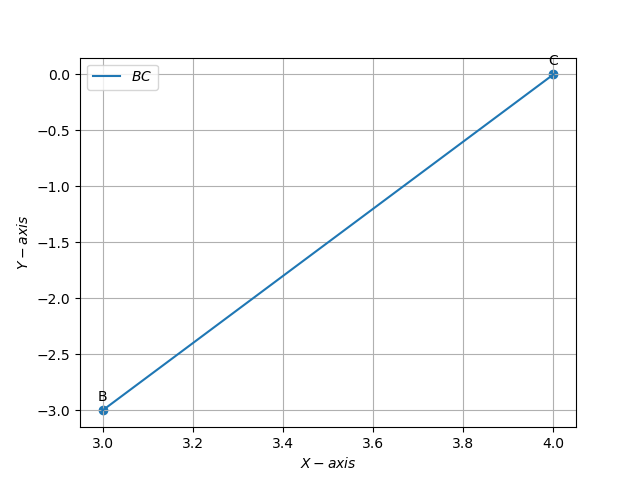
\includegraphics [width=\columnwidth]{figs/BC_line.png}
\caption{ The line $\vec{BC}$ plotted}
\label{fig:line BC}
\end{figure}

\begin{align}
	\implies \vec{CA:} \myvec{-4 & 9}\vec{x} &= -16
\end{align}
\begin{figure}[H]
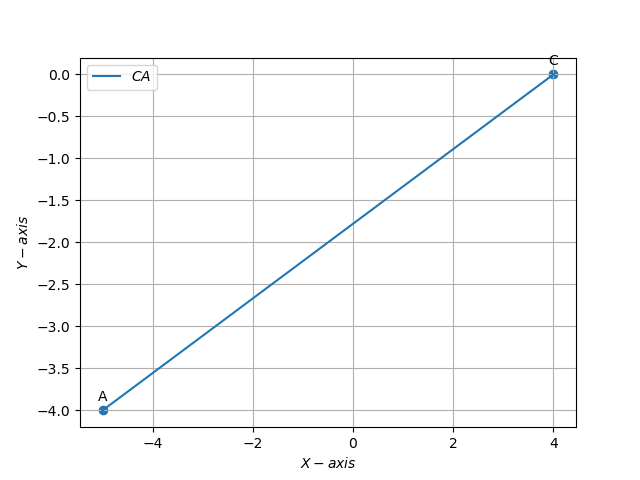
\includegraphics [width=\columnwidth]{figs/CA_line.png}
\caption{ The line $\vec{CA}$ plotted}
\label{fig:line CA}
\end{figure}
\item The area of $\triangle ABC$ is defined as
\begin{align}
\frac{1}{2}\norm{{\brak{\vec{A}-\vec{B}}\times {\brak{\vec{A}-\vec{C}}}}}
\end{align}
where,
\begin{align}
\vec{A}\times\vec{B} \triangleq \mydet{-5 & 3 \\-4& -3}
\end{align}
Find the area of $\triangle ABC$.\\
\solution\\
Given,
\begin{align}
 \vec{A} = \myvec{-5\\-4};
 \vec{B} = \myvec{3\\-3};
 \vec{C} = \myvec{4\\0}
 \end{align}
 \begin{align}
 \vec{A}-\vec{B} &= \myvec{-5\\-4} - \myvec{3\\-3} = \myvec{-8\\-1}\\
 \vec{A}-\vec{C} &= \myvec{-5\\-4} - \myvec{4\\0} = \myvec{-9\\-4}\\
\therefore(\vec{A}-\vec{B})\times(\vec{A}-\vec{C}) 
 &= \mydet{-8 & -9\\-1 & -4}\\
 &= \brak{-8 \times -4} - \brak{-9 \times -1}\\ &= 32 - 9\\ &= 23\\
 \implies\frac{1}{2}\norm{(\vec{A}-\vec{B})\times(\vec{A}-\vec{C})} &= \frac{1}{2}\norm{23}= \frac{23}{2}
\end{align}
\item Find the angles $A, B, C$ if
    \label{prop:angle2d}
    \begin{align}
    \label{eq:angle2d}
    \cos A \triangleq
\frac{\brak{\vec{B}-\vec{A}}^{\top}\brak{{\vec{C}-\vec{A}}}}{\norm{\vec{B}-\vec{A}}\norm{\vec{C}-\vec{A}}}
\end{align}
\solution\\
From the given values of $\vec{A},\vec{B},\vec{C}$,\\
\begin{enumerate}
 \item Finding the value of angle $A$
\begin{align}
 \vec{B}-\vec{A} &=\myvec{8\\1}
\end{align}
and 
\begin{align}
 \vec{C}-\vec{A} &= \myvec{9\\4}
\end{align}
also calculating the values of norms
\begin{align}
 \norm{\vec{B}-\vec{A}} &= \sqrt{65}\\
 \norm{\vec{C}-\vec{A}} &= \sqrt{97}
\end{align}
and by doing matrix multiplication we get,
\begin{align}
\begin{split}
 (\vec{B}-\vec{A})^{\top}(\vec{C}-\vec{A}) &= \myvec{8&1}\myvec{9\\4} = 76
\end{split}
\end{align}
So, we get
\begin{align}
 \cos{A} &= \frac{76}{\sqrt{65} \sqrt{97}}\\
 &= \frac{76}{\sqrt{6305}}\\
 \implies A& = \cos^{-1}{\frac{76}{\sqrt{6305}}}
\end{align}
\item Finding the value of angle B
\begin{align}
 \vec{C}-\vec{B} &=\myvec{ 1\\3}
\end{align}
and 
\begin{align}
 \vec{A}-\vec{B} &= \myvec{-8\\-1}
\end{align}
also calculating the values of norms
\begin{align}
 \norm{\vec{C}-\vec{B}} &= \sqrt{10}\\
 \norm{\vec{A}-\vec{B}} &= \sqrt{65}
\end{align}
and by doing matrix multiplication we get,
\begin{align}
\begin{split}
 (\vec{C}-\vec{B})^{\top}(\vec{A}-\vec{B}) &= \myvec{1&3}\myvec{-8\\-1} = -11
\end{split}
\end{align}
So, we get 
\begin{align}
	\cos{B} &= \frac{-11}{\sqrt{10} \sqrt{65}}\\
 &= \frac{-11}{5\sqrt{26}}\\
 \implies B& = \cos^{-1}{\frac{-11}{5\sqrt{26}}}
\end{align}

\item Finding the value of angle C
\begin{align}
 \vec{A}-\vec{C} &=\myvec{-9\\-4}
\end{align}
and 
\begin{align}
 \vec{B}-\vec{C} &= \myvec{-1\\-3}
\end{align}
also calculating the values of norms
\begin{align}
 \norm{\vec{A}-\vec{C}} &= \sqrt{97}\\
	\norm{\vec{B}-\vec{C}} &= \sqrt{10}
\end{align}
and by doing matrix multiplication we get,
\begin{align}
\begin{split}
 (\vec{A}-\vec{C})^{\top}(\vec{B}-\vec{C}) &= \myvec{-9&-4}\myvec{-1\\-3}\\
 &= 21
\end{split}
\end{align}
so, 
\begin{align}
\cos{C} &= \frac{21}{{\sqrt{97}} \sqrt{10}}\\
 &= \frac{21}{\sqrt{970}}\\
\implies C &= \cos^{-1}{\frac{21}{\sqrt{970}}}
\end{align}
\end{enumerate} 
All codes for this section are available at 
\begin{lstlisting}
       geometry/Triangle/Vectors/codes/Triangle_sides.py
\end{lstlisting}
\end{enumerate}
\backmatter
\appendix
\latexprintindex
\end{document}
